\documentclass[../masterarbeit.tex]{subfiles}
\begin{document}
	




\subsection{Feature Selection}
This section describes the results of the feature selection process of the study. It is divided into two parts. The first part is more about figuring out which meteorological data columns have a huge impact on predicting avalanches in order to create additional features. For this purpose, a decision tree classifier is used and the features classified as significant by this classifier are added to the data set for a number of days in the past.
The second part of the feature selection process is to find the approximately optimal feature set for each of the three machine learning models, trained for avalanche prediction in this study as well as to limit the number of features. For this purpose, a genetic algorithm is used to select the three features subsetssd. The two parts are described in detail in the following subsections.



\subsubsection{Decision Tree}

\begin{figure}[h]
    \centering
    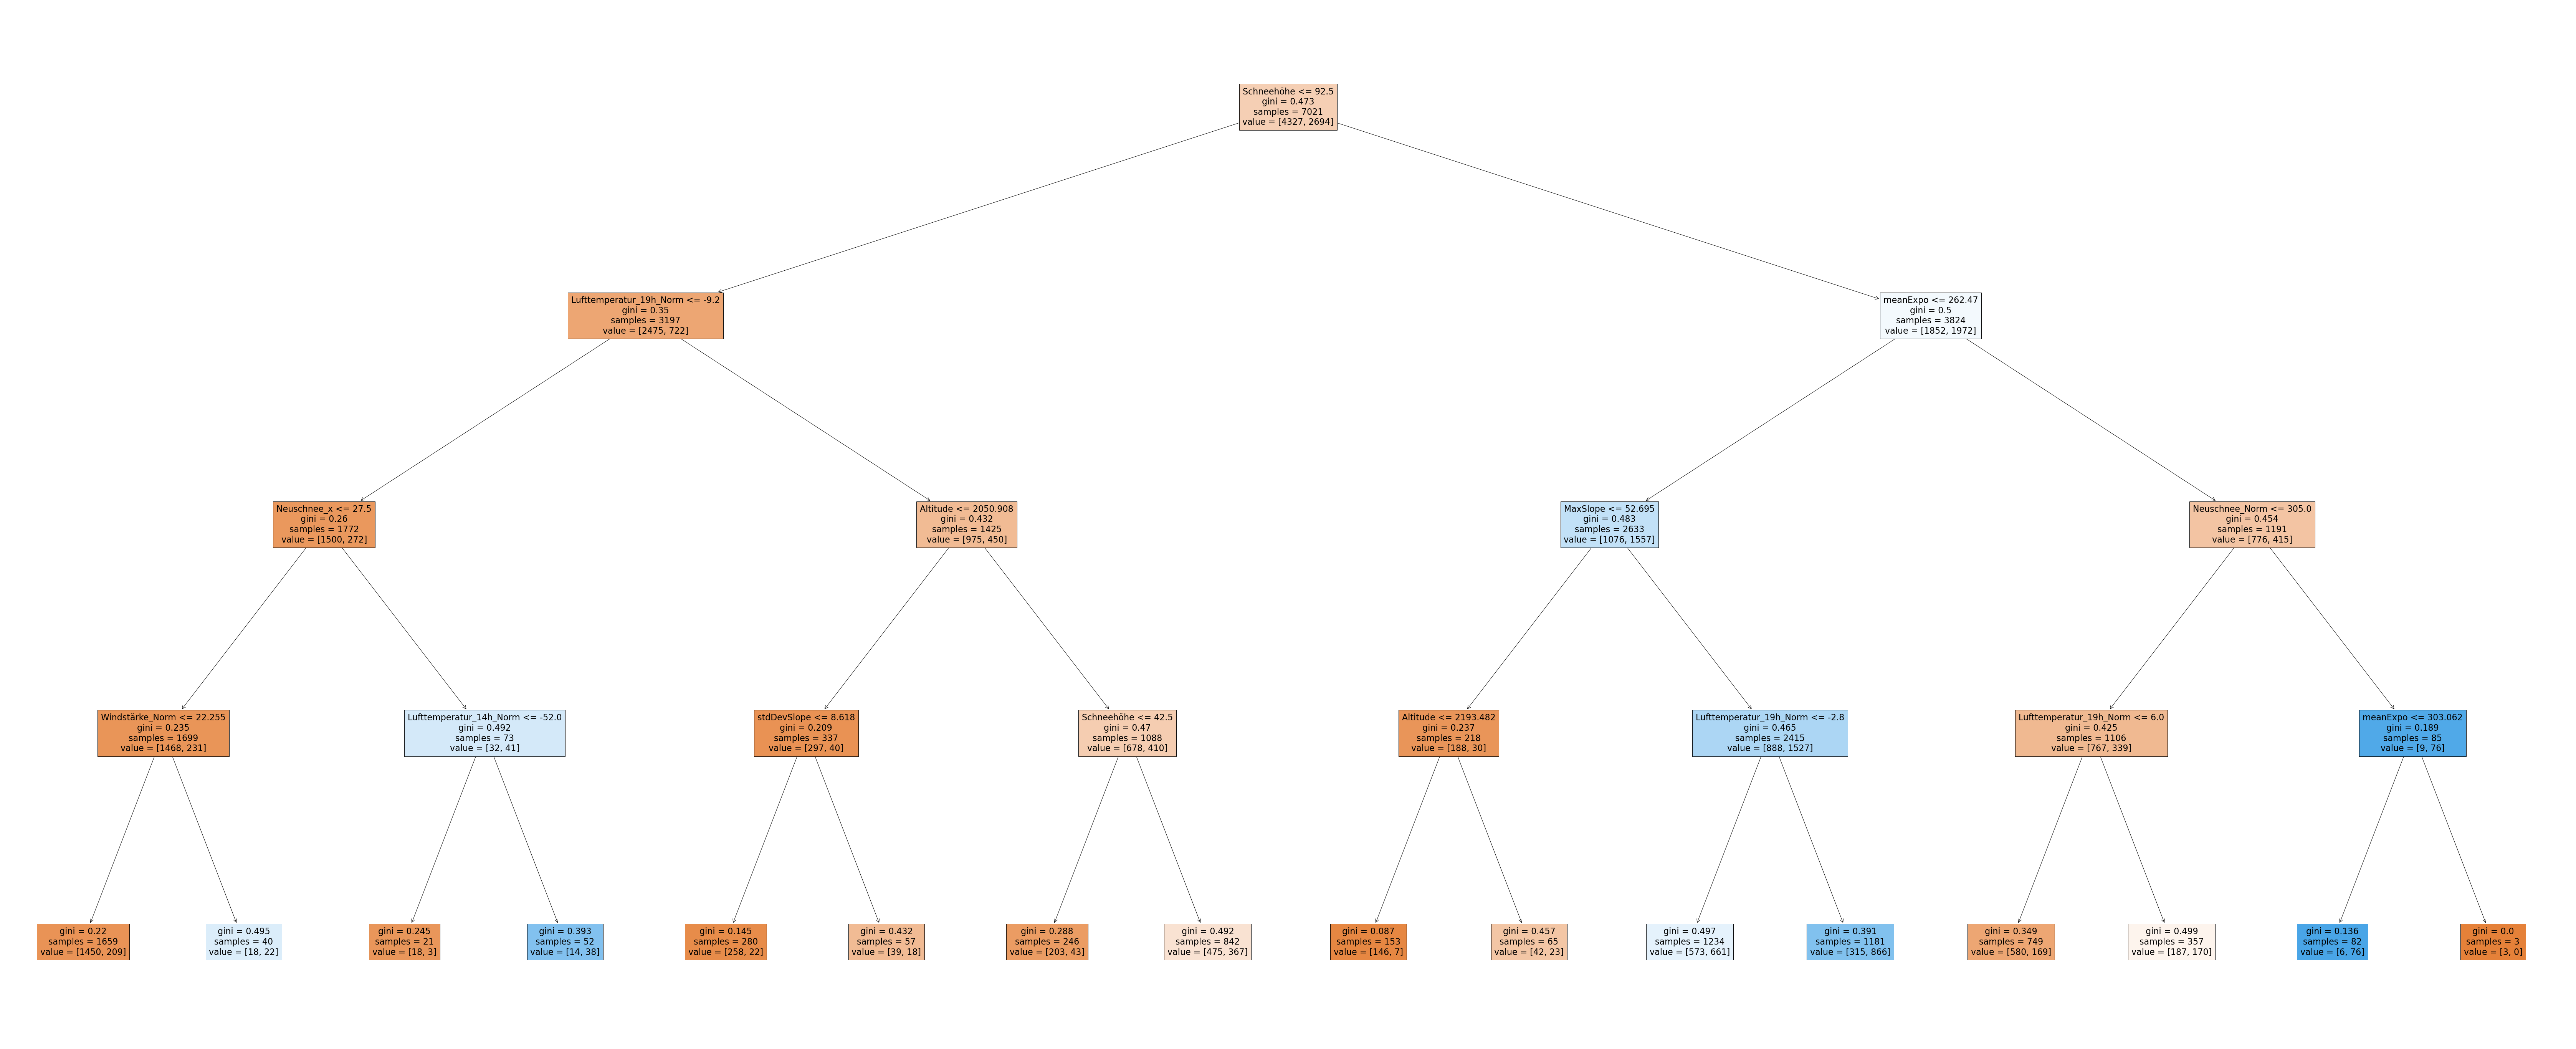
\includegraphics[scale=0.07]{avalanche_decision_tree.png}
    \source{created by the author}
    \caption{Decision Tree with a depth of 4 trained with the avalanche dataset described in section 4.1.5.}
\end{figure}

To gain an understanding of the importance of the individual data columns, a decision tree was trained using the data set created in section 4.1.5. Figure 18 shows a visualization of this tree. The nodes show wich features are used by the decision tree to create rules that are used for splitting the dataset. therefore, the features in higher-level nodes are the ones with the highest importance for the classification.
For the purpose of this task the decision tree algorithm from the python library Scikit-learn was used \textcite[]{Scikit-learn-decision-tree-classifier:2022}. The classifier model was used with a max depth of 5 and all other parameters left at the default values.
Since feature selection, as described in chapter 3.1, is mainly about reducing the size of the dataset and removing irrelevant features to improve performance, the following procedure is rather unusual. 
The dataset contains only few meteorological data of the past days. Since this data can be crucial for the prediction of avalanches, the decision tree is used in this case to find the meteorological data with the highest priority for the decision tree. 
Therefore, the main reason for creating a decision tree model in context of this master thesis is to add additionally data columns for the past two and four days to the dataset with the meteorological features used by the tree. Chawla, M. and Singh, A. \textcite[]{nhess-2021-106} used a similar approach for their study. The visualization of the decision tree model trained for this reason is displayed in figure 16. As represented in that figure, the meteorological features wich are ranked by the decision tree model as features of great importance are the following: Lufttemperatur\_19h\_Norm, Lufttemperatur\_19h , Neuschnee\_x (new snow), Windstärke\_Norm, Lufttemperatur\_14h\_Norm.
The sum of normalized new snow in the period of the last two and last four days are added as two new columns to the dataset, because this feature describes the quantity of new snow it can be added as the sum and represent the full two or four days in one new data column without losing any information.
The mean normalized air temperature and the normalized wind speed are added to the dataset for each day of the last four days. For these features the sum could not be taken, because they have fixed values and do not describe the quantity of something. To get a higher significance per column and less additional columns per day, the mean value of the normalized air temperature was calculated for each day out of the columns Lufttemperatur\_7h\_Norm, Lufttemperatur\_14h\_Norm as well as Lufttemperatur\_19h\_Norm.  The values could also be added with the mean value of the last two or four days, but In this case, the significance of the values for the individual days would be limited. The four days at the beginning of a winter interval do not have at least four previous days so every value of the Lufttemperatur and Schneehöhe where no day and therefore no data is available, the columns value is set to 0.0 for this sample. The same happens with the columns for new snow in the last two and four days, if there is not at least one preceding day. This is important because otherwise either nan values are present in the samples or the samples have to be removed to enable the training of the machine learning models. Therefore this measure is essential in order not to lose the data samples.
In total, ten new columns were added to the data set for the purpose of getting longer-term information on the meteorological conditions in the study area. The total avalanche dataset now has 56 features of which 40 are meteorological. The number of samples is the same as after data preparation, since none had to be discarded. Table 3 represents all new additionally included feature columns in combination with the corresponding descriptions, to give an overview about the new features. In the table it can be seen that out of the 10 additional features 2 are new snow related features, 4 are windspeed representing features and 4 are air temperature features.\\
Whether this additional information from the machine learning models is relevant for the prediction of avalanches will be shown in the next chapter about the results of the actual feature selection, which is performed individually for the three different classifications models using a genetic algorithm.



\begin{table}
    \centering
    \begin{tabular}{|l|l|}
    \hline
    	Column Name & Description \\ \hline
        Neuschnee\_last2 & The new snow fallen in the last two days before the current \\ \hline
        Neuschnee\_last4 & The new snow fallen in the last four days before the current \\ \hline
        windstaerke\_last1 & The wind speed on the day before the current \\ \hline
        windstaerke\_last2 & The wind speed two days before the current \\ \hline
        windstaerke\_last3 & The wind speed three days before the current \\ \hline
        windstaerke\_last4 & The wind speed four days before the current \\ \hline
        Lufttemperatur\_last1 & The air temperature one day before the current \\ \hline
        Lufttemperatur\_last2 & The air temperature two days before the current \\ \hline
        Lufttemperatur\_last3 & The air temperature three days before the current \\ \hline
        Lufttemperatur\_last4 & The air temperature four days before the current \\ \hline
    \end{tabular}
    \caption{The 10 additional feature columns in combination with their descriptions}
\end{table}









\subsubsection{Genetic Algorithm}

To get an optimal selection of features for the particular machine learning algorithms the three models Logistic Regression, Support Vector Machine and Linear Discriminant Analysis were trained repeatedly by the use of a Genetic Algorithm in the purpose of features selection. The goal of this task is to get a set of less features, which are selected as optimal as possible for the application with the corresponding machine learning model. As described in detail in section 3.1.2 the Genetic Algorithm is based on natural selection and tries to take the best features from generation to generation into the new population. So that the selection approaches the optimal data set for the respective algorithm. \\
The library contains two main genetic algorithms one for hyper-parameter optimization and the second for the task of feature selection \textcite[]{Sklearn_genetic_feature_docu:2022}. For this task the feature selection version, wich is called GAFeatureSelectionCV is used.

In purpose to use standardized feature set, the used estimator in all three runs for the different models is a pipeline with a data normalization scaler and the respective machine learning algorithm. As mentioned in section 3.1, the StandardScaler function from the Python library Sklearn is used as normalization scaler. \\







The parameters of the genetic algorithm are the same for all three machine learning models. As the first parameter the cross validation is set to a 10 fold, for the scoring of the fitness value is the accuracy score is used, the number of how many individuals are in the starting population is set to 60, the stopping criteria is the maximum generation value of 50, wich means the algorithm calculates 50 generations until it stops the process. The number of parallel running jobs is set to -1 one which stands for using all processors, therefore the learning process of the estimator and the calculation of the score are parallelized via the splitting of the cross-validation. The verbose value was set to True to reflect the progress of the algorithm in terms of the metrics of the optimization routine, as shown in Table 4 for the last generation of optimization of the Logistic Regression model. The probability that the crossover operation is performed between two individuals is left at the default value of 0.2. Also the value of the probability for child mutation is left to its default value of 0.8. The number of individuals wich perform tournament selection also remains at the default value of 3. The last parameter to mention is the maximum number of features to be selected. This value is set to None to get all features, which the algorithm thus assigns as important. All other parameters of the genetic algorithm that can be adjusted are left at their default values. \autocites{Sklearn_genetic_feature_docu:2022}
The output metrics of the genetic algorithms are shown in table 4, 5 and 6 for the three different results \textcite[]{Sklearn_genetic_feature_docu_metrics:2022}: 
\begin{itemize}
	\item "gen": The number of the generation.
	\item "nevals": The value of the population used for the current generation.
	\item "fitness": The average fitness score, wich in the case of this study is the accuracy score, over the cross-validation folds results.
	\item "fitness\_std": The representation of the standard deviation of the cross-validation accuracy.
	\item "fitness\_min": The minimum fitness score of the cross-validation folds.
	\item "fitness\_max": the maximum fitness score of the cross-validation. 
\end{itemize}


\begin{table}[!ht]
    \centering
    \begin{tabular}{|l|l|l|l|l|l|}
    \hline
        "gen" & "nevals" & "fitness" & "fitness\_std" & "fitness\_max" & "fitness\_min"  \\ \hline
        50 & 120 & 0.733517 & 0.000460338 & 0.733647 & 0.730656 \\ \hline
    \end{tabular}
    \caption{The metrics of the last generation calculated by the genetic algorithms optimization routine while optimizing the dataset for the Logistic Regression model.}
\end{table}
First of the three models, the Logistic Regression model was trained by the genetic algorithm. As a result the genetic algorithm created a subset of 20 features as a best approximation to the optimal subset for the logistic regression model. 
As shown in Table 4, the process of optimizing the data set for the Logistic Regression model was completed with the 50th generation with an average accuracy of 0.733517. Where the lowest value of 10-fold cross-validation is 0.730656, the highest is 0.733647, and the standard deviation of all values in the series is 0.000460338.
Table 5, which contains a count of the selected features, shows the subset of selected features for the Logistic Regression Model contains the two factors windstaerke\_last3 and
Lufttemperatur\_last4, wich were added to the dataset by the previous process explained in section 4.2.1, as shown in Table 3. The optimized subset for the Logistic Regression model includes in total 9 meteorological features, five snowpack related columns as well as all of the six topographical factors.\\
\begin{table}
    \centering
    \begin{tabular}{|l|l|l|l|l|l|}
    \hline
        "gen" & "nevals" & "fitness" & "fitness\_std" & "fitness\_max" & "fitness\_min"  \\ \hline
        50 & 120 & 0.735865 & 0.00171288 & 0.737352 & 0.728662 \\ \hline
    \end{tabular}
    \caption{The metrics of the last generation calculated by the genetic algorithms optimization routine while optimizing the dataset for the LDA model.}
\end{table}
The second approximately optimal subset was calculated for the LDA model by the genetic algorithm. 
After passing the 50 generation, the second run of the genetic algorithm to obtain an optimized set for the LDA was completed with an average accuracy of 0.735865. The lowest value of the series of accuracy scores in this case was 0.728662, the highest 0.737352, and the standard deviation of the entire series was 0.00171288. The list of values can be found in table 5. 
The resulting subset includes 24 features. Nine of the selected columns are meteorological features, of which the five columns Neuschnee\_last4, Neuschnee\_last2, windstaerke\_last1, windstaerke\_last2 and Lufttemperatur\_last4 are from the new features added in section 4.2.1. The genetic algorithm also included all six topographic factors as well as three snowpack related features in the subset.\\
\begin{table}
    \centering
    \begin{tabular}{|l|l|l|l|l|l|}
    \hline
        "gen" & "nevals" & "fitness" & "fitness\_std" & "fitness\_max" & "fitness\_min"  \\ \hline
        50 & 120 & 0.768267 & 0.00159737 & 0.768972 & 0.762988 \\ \hline
    \end{tabular}
    \caption{The metrics of the last 10 generations calculated by the genetic algorithms optimization routine while optimizing the dataset for the SVM model.}
\end{table}
The last subset, wich is created by the genetic algorithm optimized for the SVM is a combination of 25 features. Therefor, this subset is the largest of the three. It includes 15 meteorological, five snowpack related and five topographical features.  Also for the optimized subset for the SVM, the two new meteorological factors of the past days Neuschnee\_last4 and Lufttemperatur\_last4 were selected. 
The genetic algorithms last generation shows an accuracy of 0.768267 and completes the features selection process with the highest value of the three machine learning models. The smallest accuracy score measured in the 10-fold cross-validation series is 0.762988. The highest accuracy score is 0.768972 and the standard derivation is 0.00159737. While the the final values for the LDA and the Logistic Regression model after feature selection are close to each other, the values of the SVM model are higher than both of the other models. \\
\begin{figure}[h]
    \centering
    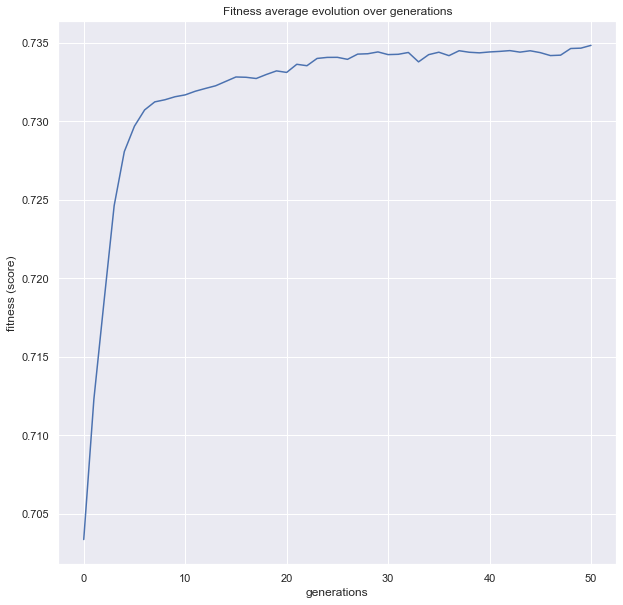
\includegraphics[scale=0.23]{LR_GA_evolution.png}
    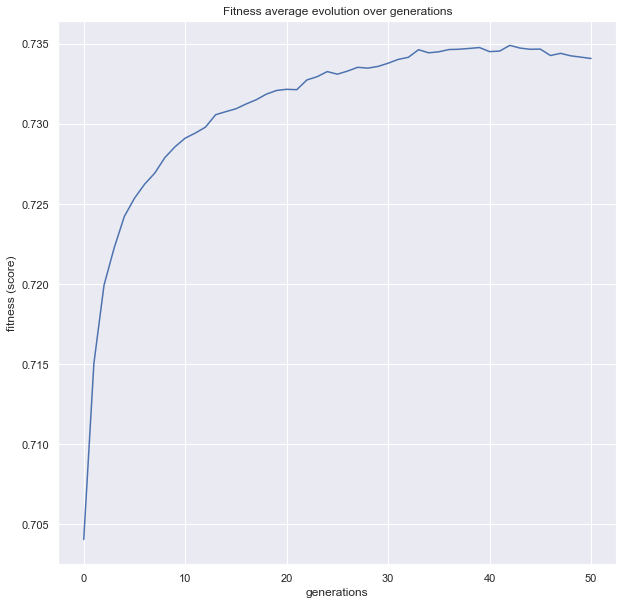
\includegraphics[scale=0.23]{LDA_GA_evolution.png}
    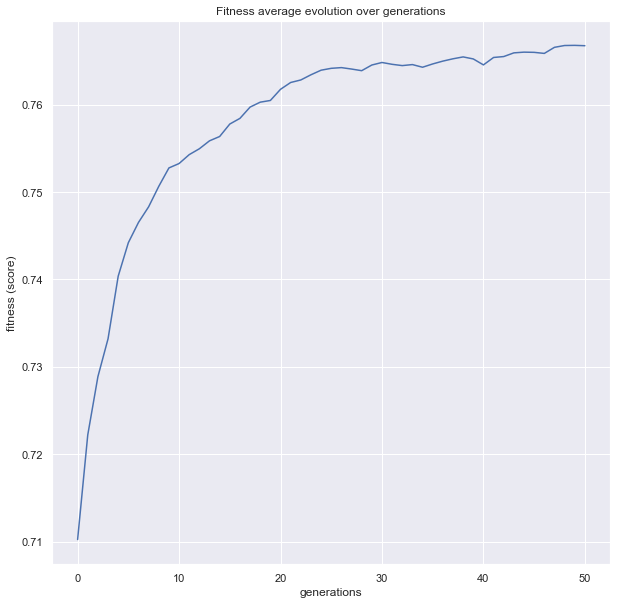
\includegraphics[scale=0.23]{SVM_GA_evolution.png}
    \source{created by the author}
    \caption{The fitness evolution increase over 50 generations created by the genetic algorithm for the Logistic Regression, LDA and SVM models.}
\end{figure}
The three graphs pictured in figure 17 show the increase of the fitness score over the 50 generations, created by the genetic algorithm. The left graph shows the fitness evolution of the Logistic Regression model. It started an average fitness score over the 10-fold cross validation of 0.704242 increased in the first 6 generations and completed the process with the value of 0.733517. The graph in the middle of the three figures represents the fitness evolution of the LDA. As the graph shows, the fitness score in this case increases more continuously over the entire 50 generation. It is also noticeable,  that it drops again somewhat towards the end. The application of the genetic algorithm to the LDA started with a fitness score of 0.703853 and ended with a value of 0.735865. The fitness evolution of the SVM model increased while the feature selection process with the genetic algorithm from an average accuracy of 0.709667 in the first generation to 0.768267 in the 50st generation.\\
\begin{table}[!ht]
    \centering
    \begin{tabular}{|l|l|l|}
    \hline
        Logistic Regression & LDA & SVM \\ \hline
        Schneehöhe & Schneehöhe & Schneehöhe \\ \hline
        Lufttemperatur\_7h\_Gew & Niederschlag & Lufttemperatur\_7h \\ \hline
        Lufttemperatur\_14h & Lufttemperatur\_7h & Lufttemperatur\_14h\_Norm \\ \hline
        Lufttemperatur\_14h\_Gew & Lufttemperatur\_7h\_Gew & Lufttemperatur\_14h\_Gew \\ \hline
        Lufttemperatur\_19h & Lufttemperatur\_14h\_Norm & Lufttemperatur\_19h \\ \hline
        Schneetemperatur & Lufttemperatur\_14h\_Gew & Lufttemperatur\_19h\_Norm \\ \hline
        Schneetemperatur\_Gew & Lufttemperatur\_19h & Lufttemperatur\_19h\_Gew \\ \hline
        Windstärke & Schneetemperatur & Schneetemperatur \\ \hline
        Einsinktiefe\_Norm & Windrichtung\_Gew & Schneetemperatur\_Norm \\ \hline
        Einsinktiefe\_Gew & Windstärke\_Norm & Schneetemperatur\_Gew \\ \hline
        Wetter\_akt & Einsinktiefe\_Norm & Windstärke \\ \hline
        Neuschnee\_Norm & Wetter\_akt & Windstärke\_Gew \\ \hline
        windstaerke\_last3 & Neuschnee\_Norm & Einsinktiefe\_Gew \\ \hline
        Lufttemperatur\_last4 & Neuschnee\_last4 & Wetter\_akt \\ \hline
        meanExpo & Neuschnee\_last2 & Wetter\_gestern \\ \hline
        meanSlope & windstaerke\_last1 & Wolken \\ \hline
        stdDevSlope & windstaerke\_last2 & Neuschnee\_x \\ \hline
        MinSlope & Lufttemperatur\_last4 & Neuschnee\_Norm \\ \hline
        MaxSlope & meanExpo & Neuschnee\_last4 \\ \hline
        Altitude & meanSlope & Lufttemperatur\_last4 \\ \hline
         & stdDevSlope & meanExpo \\ \hline
         & MinSlope & meanSlope \\ \hline
         & MaxSlope & MinSlope \\ \hline
         & Altitude & MaxSlope \\ \hline
         &  & Altitude \\ \hline
    \end{tabular}
    \caption{The features selected by the genetic algorithm for the three machine learning models, Logistic Regression, LDA and SVM}
\end{table}
The resulting three optimized datasets are represented in Table 7. The table contains one column per machine learning model. In these columns, the data sets are assigned to the corresponding machine learning models. By analyzing the datasets in the table, similarities of the selected features for the three algorithms are recognizable. The columns Schneehöhe, Lufttemperatur\_14h\_Gew, Lufttemperatur\_19h, Schneetemperatur, Wetter\_act, Neuschnee\_Norm, Lufttemperatur\_last4 are meteorological data that are included in all three optimized datasets, which suggests that they are of higher importance for the prediction of avalanches. Also the different features wich represent the air temperature at various points in time are represented several times in all subsets. Thus, 6 features are present in the set optimized for the logistic regression model, 5 in the set for the LDA, and 7 in the optimized subset of the SVM model features representing the air temperature. This suggests a correlation between air temperature and avalanche prediction for all three sets. 
Furthermore, the topographic factors are fully present in the Logistic Regression and Linear Discriminant Analysis set and in the Support Vector Machine set five out of six features are included, whereas the standard deviation of the slope is excluded here. 
In comparison to the study "Snow avalanche hazard prediction using machine learning methods", mentioned in Chapter 2, in this study the altitude is represented in all three datasets, while the study ranked the altitude as the last important feature for avalanche prediction \textcite[]{Bahram:2019}.
It can be concluded that an accurate definition of slopes based on topographic factors is related to the quality of avalanche prediction.









\end{document}